\documentclass[a4paper,12pt]{article}
\usepackage{blindtext}
\usepackage[utf8]{inputenc}
\usepackage{graphicx}
\usepackage{enumitem}
%\usepackage{pgfplotstable}
%\usepackage{booktabs}

\begin{document}
\begin{titlepage}
\center

\textsc{\LARGE Architectural Requirements}\\[1.5cm]
\textsc{\Large Project: Traffic Camera Image Analysis}\\[1.5cm]
\textsc{\large Client: DPSS, CSIR}\\[0.5cm]
\textsc{\large Team: Quadcore Productions}\\[0.5cm]

\begin{minipage}{0.4\textwidth}
\begin{flushleft} \large
\textbf{Author(s):}\\
Mpho \textsc{Baloyi}\\
Hlengekile \textsc{Jita}\\
Mayimela \textsc{Moses}\\
Mbhele \textsc{Themba}\\
\end{flushleft}
\end{minipage}
~
\begin{minipage}{0.4\textwidth}
\begin{flushright} \large
\textbf{Student number(s):} \\
14133670\\ % Student number
14077893\\
14019702\\
14007950\\
\end{flushright}
\end{minipage}\\

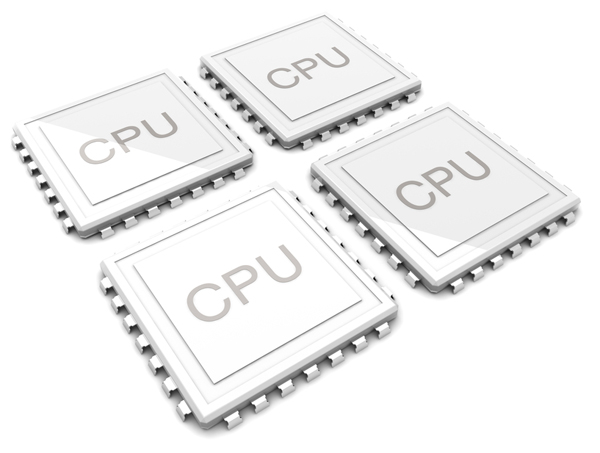
\includegraphics[width=\textwidth]{2012-quad-core-phones.jpg}

{\large University of Pretoria, Department of Computer Science}\\

{\large 29 July 2016}\\[3cm]

\vfil

\end{titlepage}

\newpage
\tableofcontents
\newpage

\newpage
\section{Version History}
%\begin{table}[]
%\begin{center}
%    \caption{Document History}
%    \pgfplotstabletypeset[
%      multicolumn names, % allows to have multicolumn names
%      col sep=comma, % the seperator in our .csv file
%      display columns/0/.style={
%		column name=$Value 1$, % name of first column
%		column type={S},string type}, 
%      display columns/1/.style={
%		column name=$Value 2$,
%		column type={S},string type},
%	  display columns/2/.style={
%		column name=$Value 3$,
%		column type={S},string type},
%	  display columns/3/.style={
%		column name=$Value 2$,
%		column type={S},string type},
%	  every head row/.style={
%		before row={\toprule},
%		after row={\midrule}},
%	  every last row/.style={after row=\bottomrule},
%    ]{versionTable.csv} % filename/path to file
%  \end{center}
%\end{table}
\newpage

\section{Introduction}
This document describes the functional requirements and application design of the Traffic Camera Image Analysis System. The target system will run on a web server  and be accessed by users on an Android Application which will provide the users with the necessary functionality to access real-time traffic information that assists them with things such as avoiding traffic and choosing the best alternative routes. 

In this specification, we cover the use cases, their service contracts, required functionality and process specifications of the target system. The above, will be built on over time as the software is developed, as we are following an agile development methodology. In addition the domain model of the application as a whole will be provided.
\section{Vision}
For this project we aim to achieve a system that makes use of images obtained from highway cameras to provide users with up-to-date real-time traffic information. The system should simplify the user's travels by providing traffic information and notifying them before they depart of traffic conditions, calculating arrival times based on traffic conditions and help them select the most suitable route for their trips using the traffic information and additional metrics. Our vision for the target system is that it should be reliable and perform relatively quickly, both for user satisfaction and in order to be the an up-to-date traffic information system.
\section{Background}
As a commuter, traffic is something that is a part of everyday life, and it is not one of the more pleasurable aspects of life. Already there is software in place that assists us in dealing with this problem, such as Google Maps. This software uses the crowd-sourcing of GPS data in order to provide their up-to-date traffic information.

In our system,we want to take an image analysis approach to solve the same problem. We will make use of the publicly available SANRAL highway cameras to get images. Processing these images we will perform image analysis and determine the traffic conditions in the area of a camera. Using this information we will be able to generate information pertaining to user specified routes in order to provide the information necessary to help them avoid traffic and choose the most suitable routes in order to do so.
\section{System Scope}
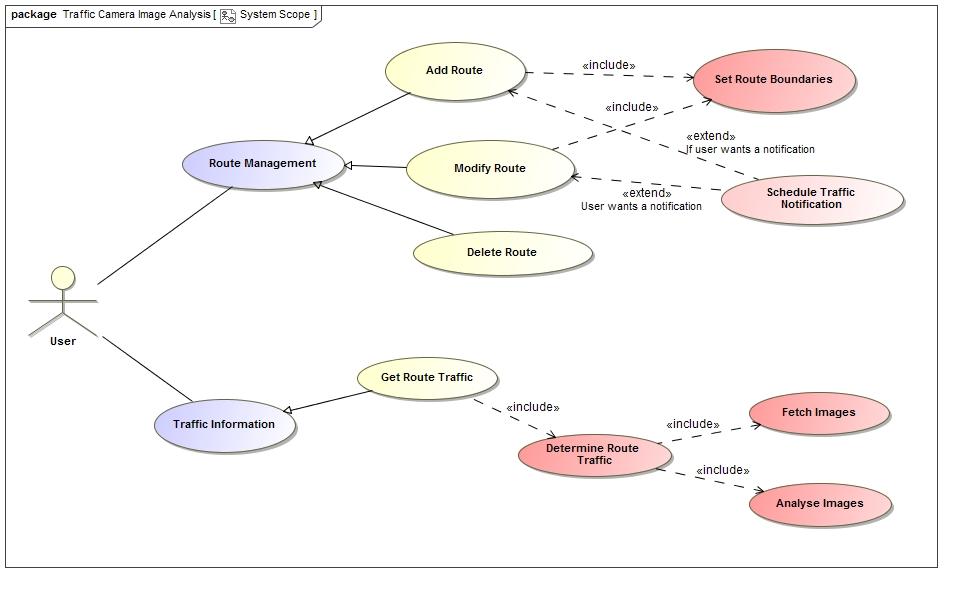
\includegraphics[width=\textwidth]{images/System_Scope.jpg}

The purpose of this system as stated earlier, is to provide the user with traffic information based on image analysis from images accessed from highway cameras. Thus the user will need to be able to access services that allow the achievement of this goal.

The scope of the system thus includes the tasks the user can access such as add route, modify route, delete route and get route traffic.
\section{Functional Requirements}
\subsection{Use Cases}
The use cases for our system are described below. These use cases are the services that provide the user of the application some value. The following uses are listed in order of prioritization:
\begin{itemize}
\item Add Route 			(Critical)
\item Get Route Traffic		(Critical)
\item Modify Route			(Critical)
\item Delete Route			(Critical)
\item Schedule Notification (Important)
\item Route Optimization 	(Nice To Have)
\end{itemize}
\subsection{Service Contracts}
For each of the above services described above, there are are pre-conditions that must be met for the service to be carried out and post-conditions that are met to indicate the successful completion of a service. In addition the service contracts indicate what exceptions will be thrown in case the service fails.

\subsubsection{Add Route}
%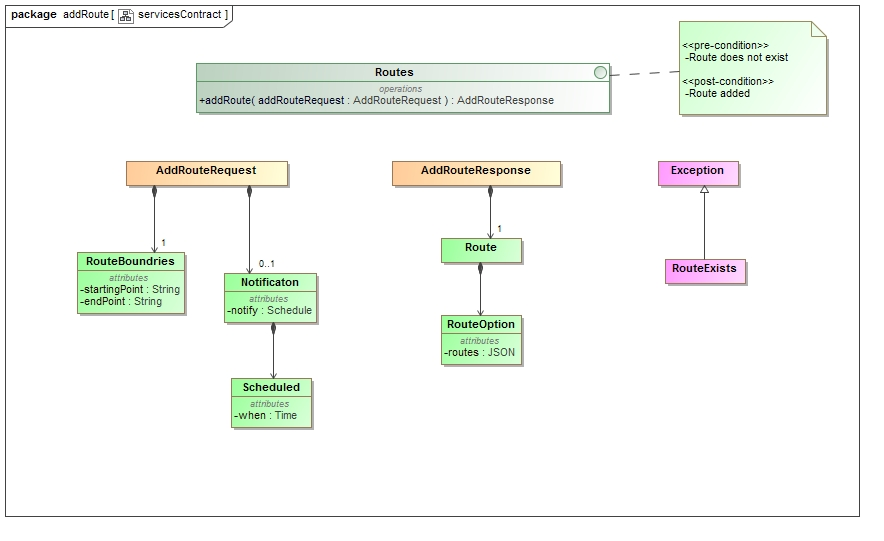
\includegraphics[width=\textwidth]{images/scAdd_Route.jpg}


\textbf{Pre-Condition: }
Valid route boundaries.\\
Route does not already exist.\\
\textbf{Post-Condition: }
New route is created and stored.\\

This use case creates a new route and stores it so that it can be used in requests for traffic information. It first checks that the route to be created is valid and does not already exist in storage, then it creates and stores the route. In the case that the route exists an exception is raised.
\subsubsection{Modify Route} 
%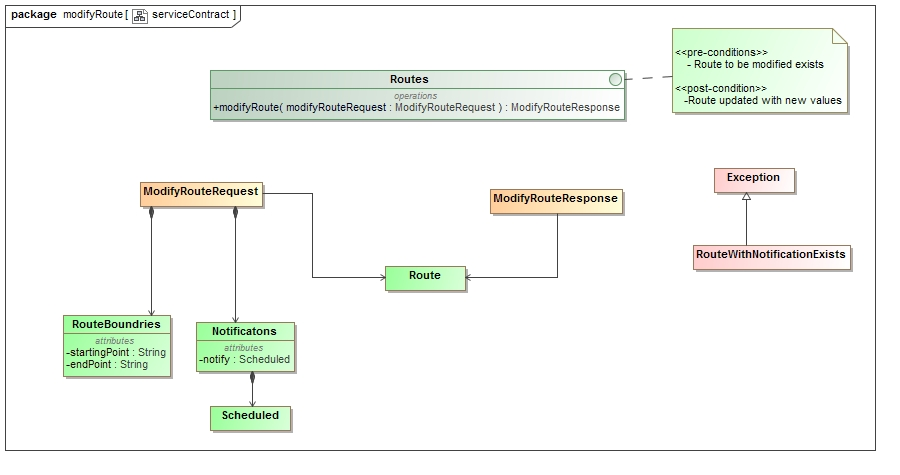
\includegraphics[width=\textwidth]{images/scModify_Route.jpg}
\textbf{Pre-Condition: }
Route exists.\\
\textbf{Post-Condition: }
Route is modified and the modified route is stored.\\

This use case makes changes to existing routes and stores the changes. In order to do this, this use case first checks if the route exists, if so it then makes the necessary changes to the route and then stores the route. If the route does not exist an exception is raised. 
\subsubsection{Delete Route}
%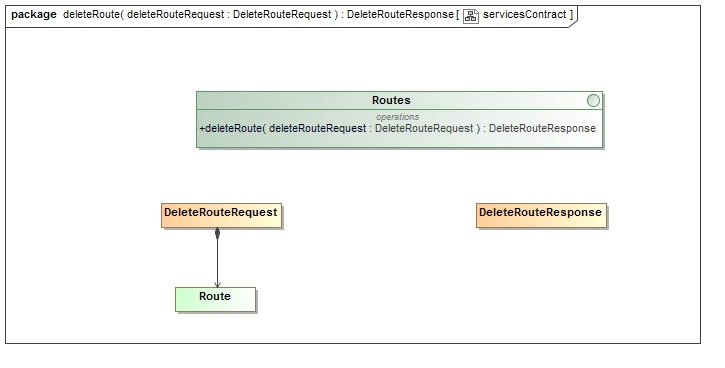
\includegraphics[width=\textwidth]{images/scDelete_Route.jpg}
\textbf{Pre-Condition: }
Route exists.\\
\textbf{Post-Condition: }
Route is removed\\
This use case removes an existing route. Before it does this it checks if the route exists in storage then removes it. In the case that the route does not exist an exception is raised.
\subsubsection{Get Route Traffic}
%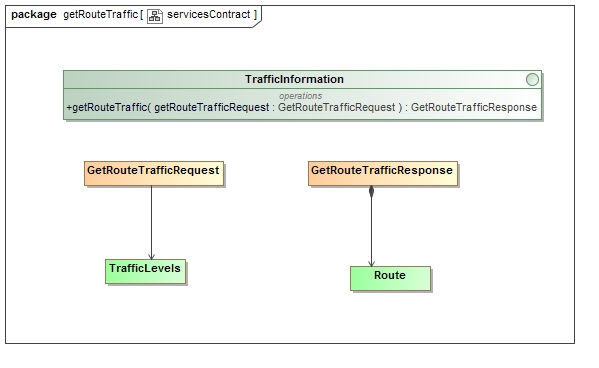
\includegraphics[width=\textwidth]{images/scDetermine_Traffic.jpg}
\textbf{Pre-Condition: }
Route consists of camera locations.\\
Camera locations on route has valid images.\\
\textbf{Post-Condition: }
Traffic information for route is generated.\\

This use case generates traffic information based on a route provided with the request. To do this it first checks if the route covers any of the camera locations, if not no traffic information is generated and an exception is raised. Otherwise it continues and retrieves the images for the camera's within the route, thereafter it checks if these images are valid, if all are invalid, no traffic information is generated, it then performs image analysis on the valid images and determine the traffic levels and generates traffic information for the route.

\subsubsection{Schedule Notification}
%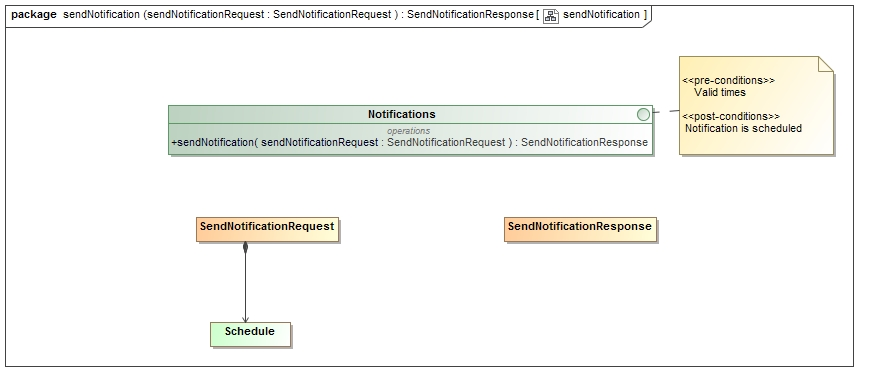
\includegraphics[width=\textwidth]{images/scSchedule_Notification.jpg}
\textbf{Pre-Condition: }
Valid times\\
\textbf{Post-Condition: }
Notification is scheduled\\

This use case allows the user to schedule notifications of traffic information at specific times. This is done by allowing the user to specify a time to be notified about a route when adding or modifying it. This time is then used to schedule automated traffic information requests.
\subsection{Required Functionality}
The use cases make use of other lower level functions in order to achieve their purpose. In the below diagrams for each high level use case, the lower level use cases that are required are described.
\subsubsection{Add Route}
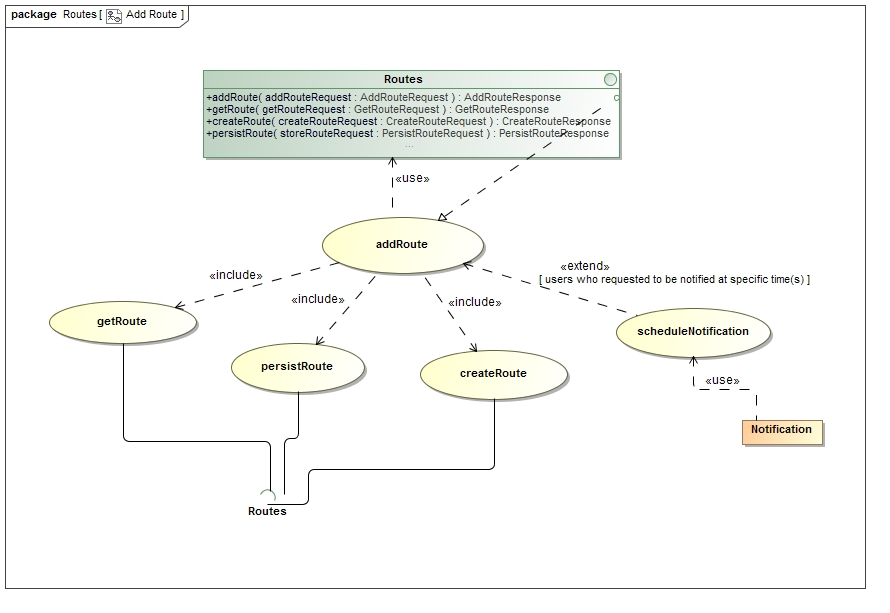
\includegraphics[width=\textwidth]{images/Add_Route.jpg}

The Add Route use case makes use of the following lower level functions to add a route to the system:
\begin{itemize}
\item \textbf{getRoute -} This checks if the route exists already or not.
\item \textbf{createRoute -} This creates a route, or a set of directions, based on the route boundaries (departure and destination points).
\item \textbf{persistRoute -} This stores the route so that it is available for later use.
\end{itemize}
\subsubsection{Modify Route} 
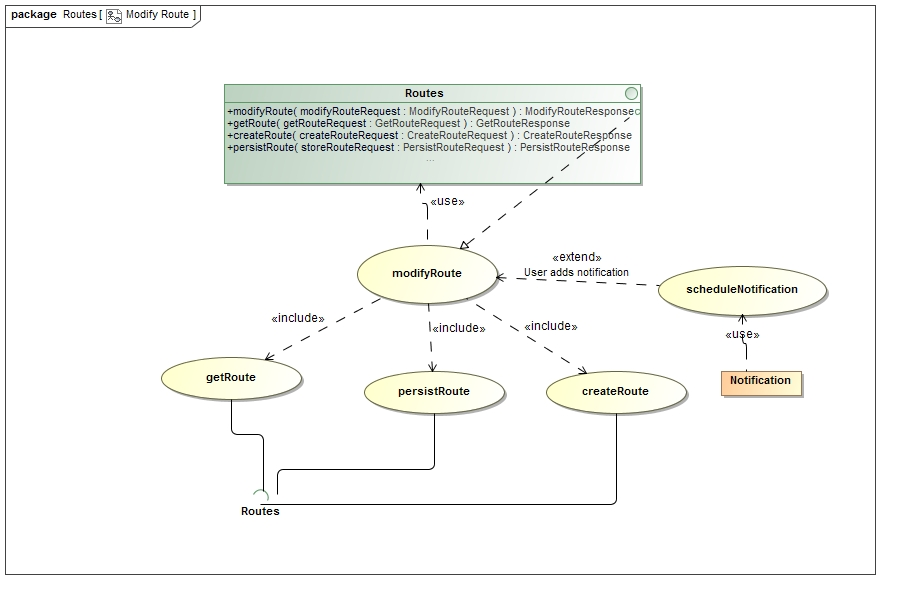
\includegraphics[width=\textwidth]{images/Modify_Route.jpg}
The Modify Route use case makes use of the following lower level functions to make changes to an already existing route.
\begin{itemize}
\item \textbf{getRoute -} This checks if the route exists already.
\item \textbf{createRoute -} This creates a route, or a set of directions, based on the route boundaries (departure and destination points). Only if the changes are in the route boundaries.
\item \textbf{persistRoute -} This stores the modified route.
\end{itemize}
\subsubsection{Delete Route}
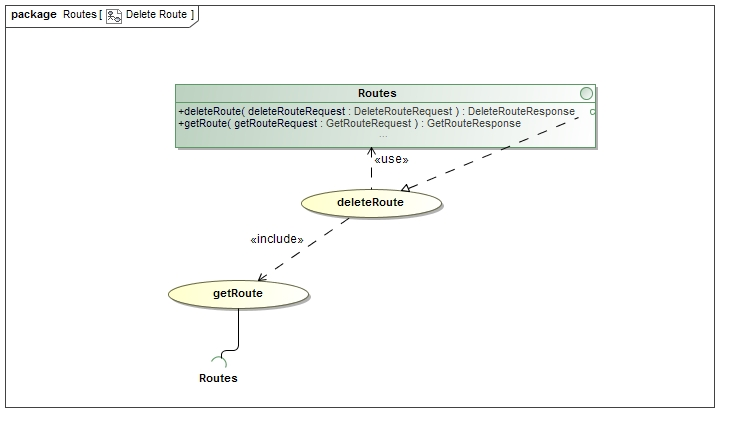
\includegraphics[width=\textwidth]{images/Delete_Route.jpg}
The Delete Route use case makes use of the following lower level functions to assist in removing the route from storage:
\begin{itemize}
\item \textbf{getRoute -} This checks if the route exists already .
\end{itemize}
\subsubsection{Get Route Traffic}
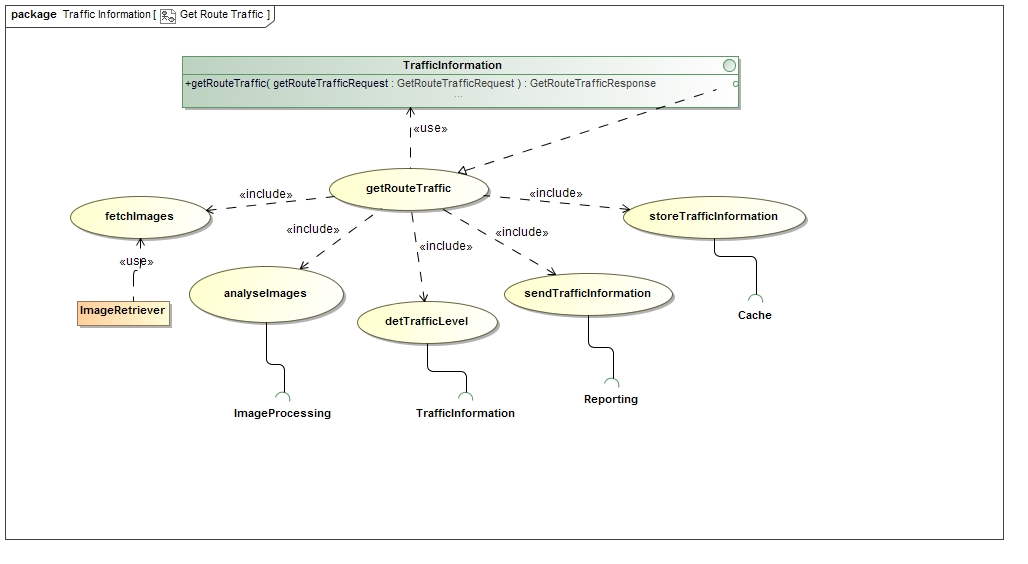
\includegraphics[width=\textwidth]{images/Get_Route_Traffic.jpg}
The Get Route Traffic use case makes use of the following lower level functions, both within and outside the Routes module to determine the traffic of a route and send it back to the user:
\begin{itemize}
\item \textbf{fetchImage -} This function fetches an image from the camera at the specified location.
\item \textbf{analyseImage -} This function performs image analysis in order to determine the traffic level in that location
\item \textbf{composeTrafficInfo -} This function composes all the traffic levels that make up the route and constructs a preliminary "traffic info report".
\item \textbf{sendTrafficInformation -} This function creates a traffic information report and sends it to the user who requested it.
\item \textbf{storeTrafficLevels -} The traffic levels are stored for any other user to be able to access it if necessary instead of performing analysis again.
\end{itemize}

\subsection{Process Specification}
This section describes the process for completing the Add Route, Modify Route and Get Route Traffic Sections.
\subsubsection{Add Route}
%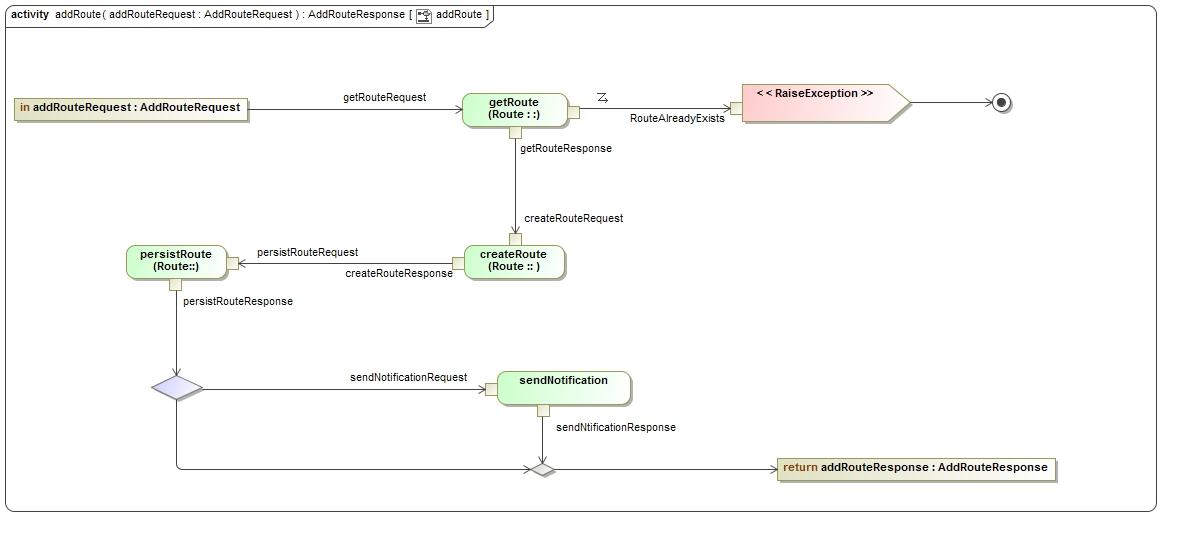
\includegraphics[width=\textwidth]{images/psAdd_Route.jpg}
\subsubsection{Modify Route}
%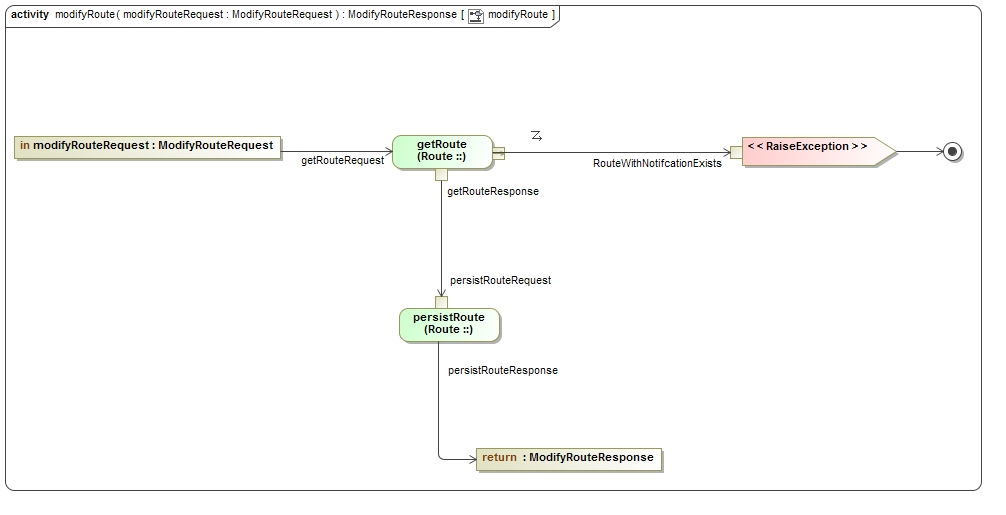
\includegraphics[width=\textwidth]{images/psModify_Route.jpg} 
\subsubsection{Get Route Traffic}
%\includegraphics[width=\textwidth]{images/psGet_Route_Traffic.jpg}

\section{Domain Model}
%\includegraphics[width=\textwidth]{images/Domain_Model.jpg}

\section{Open Issues}
Some of the issues that still need to be covered, and that still need more clarification are the following:
\begin{itemize}
\item Domain model for the modules of the system, still need further clarification on format of some data
\item Further work is to be done on the Get Route Traffic service
\item Route Optimization, currently debating the value, if any, this service might add to the system.
\end{itemize}

\end{document}